\documentclass[12pt]{exam}
\usepackage[german]{babel}
\usepackage[utf8x]{inputenc}
\usepackage{graphicx}
\usepackage{latexsym,ifthen,amssymb,amsfonts,amsmath}

\begin{document}

\include{definitions}

\pagestyle{empty}

\def\loesungen{0}
\newcommand{\lansel}[2]{#1}

\ifthenelse{\equal{\loesungen}{1}}{\printanswers}{\relax}
\renewcommand{\solutiontitle}{\noindent\textbf{L\"osung:}\enspace}
\newcommand{\loesungname}{\ifthenelse{\equal{\loesungen}{1}}{L\"osungen zu }{\relax}}

\begin{center}
\textbf{\LARGE \loesungname \lansel{\"Ubungsblatt}{Examples Sheet} 1} \\ \vspace{1ex}
\textbf{\large \lansel{zum Mathematischen Brückenkurs \\ für Naturwissenschaftler:innen}{for the preparatory mathematics course for bio- and geoscientists}} \\ \vspace{1ex}
\textbf{\large \lansel{im Wintersemester}{Winter} 2023/24} \\ \vspace{0.5cm}
\textrm{\normalsize \hfill \lansel{Dozent}{Lecturer}: Apl.Prof. Dr. G. von Hippel\hfill${}$}
\end{center}
\normalsize\vspace{0.5cm}

\ifthenelse{\equal{\loesungen}{1}}{
\begin{center}
\textbf{Die direkte Weitergabe der Musterl\"osungen an Studierende ist nicht gestattet!}
\end{center}
}{
\vspace{3ex}
}

\begin{questions}
\pointname{ P.}

%%%%%%%%%%%%%%%%%%%%%%%%%%%%%%%%%%%%%%%%%%%%%%%%%%%%%%%%%%%%%%%%%%%%%%%%%%%%%%%

\question{{\it Aussagenlogische Gesetze}}

Beweisen Sie folgende aussagenlogische Gesetze mit Hilfe von Wahrheitstafeln:
\begin{enumerate}
\item $(a\wedge(b\wedge c))\Leftrightarrow((a\wedge b)\wedge c)$
\item $(a\vee(b\vee c))\Leftrightarrow((a\vee b)\vee c)$
\item $(a\Rightarrow b)\Leftrightarrow(\neg a\vee b)$
\item $(p\Rightarrow q)\Leftrightarrow(\neg q\Rightarrow\neg p)$
\item $(r\Leftrightarrow s)\Leftrightarrow((r\Rightarrow s)\wedge (s\Rightarrow r))$
\item $(a\wedge(b\vee c))\Leftrightarrow((a\wedge b)\vee(a\wedge c))$
\item $(a\vee(b\wedge c))\Leftrightarrow((a\vee b)\wedge(a\vee c))$
\item $((p\Rightarrow q)\wedge(q\Rightarrow r)\wedge(r\Rightarrow p))\Leftrightarrow((p\Leftrightarrow q)\wedge(q\Leftrightarrow r))$
\end{enumerate}



\question{{\it Aussagen mit Quantoren}}

Übersetzen Sie folgende Aussagen in umgangssprachliche Sätze bzw. umgekehrt, wobei $s(x)$ für ``$x$ ist ein Snark'', $b(x)$ für ``$x$ ist ein Boojum'', $f(x,y)$ für ``$x$ findet $y$'' stehen möge:
\begin{enumerate}
\item $\exists x~(s(x)\wedge b(x))$
\item $\exists x~\exists y~(s(y)\wedge f(x,y))$
\item $\forall x~b(x)\Rightarrow (s(x)\wedge \neg f(x,x))$
\item Jeder Snark, der von jemandem gefunden wird, ist ein Boojum.
\item Alle Boojums sind Snarks, aber nicht alle Snarks sind Boojums.
\item Jeder Boojum wird von jemandem gefunden.
\end{enumerate}



\question{{\it Einfache Operationen mit endlichen Mengen}}

Geben Sie für die folgenden Paare von Mengen $A$, $B$ jeweils $A\cup B$, $A\cap B$, $A\backslash B$, $B\backslash A$, $A\times B$ und $B\times A$ an:\\
\parbox{0.5\textwidth}{
\begin{enumerate}
\item $A=\{1,2,3\}$, $B=\{2,4,6,8,10\}$
\item $A=\{1,2,3,4\}$, $B=A$
\end{enumerate}}\parbox{0.5\textwidth}{
\begin{enumerate}\setcounter{enumi}{2}
\item $A=\{\emptyset,\{\emptyset\}\}$, $B=\{\emptyset,\{\emptyset,\{\emptyset\}\}\}$
\item $A=\{1,2,3,4\}$, $B=\{A\}$
\end{enumerate}}



\question{{\it Venn-Diagramme -- I}}

Zeichnen Sie jeweils ein Venn-Diagram, das die folgenden Verhältnisse zwischen Mengen widerspiegelt:
\begin{enumerate}
\item $B\subset A$, $C\cap A=\emptyset$
\item $A\cap B\not=\emptyset$, $\neg((A\subseteq B)\vee (B\subseteq A)$, $C\subset A$, $C\cap B=\emptyset$
\item $B\subset A$, $C\subset B$, $D\subset A$, $D\cap B=\emptyset$
\end{enumerate}



\question{{\it Venn-Diagramme -- II}}

\begin{center}
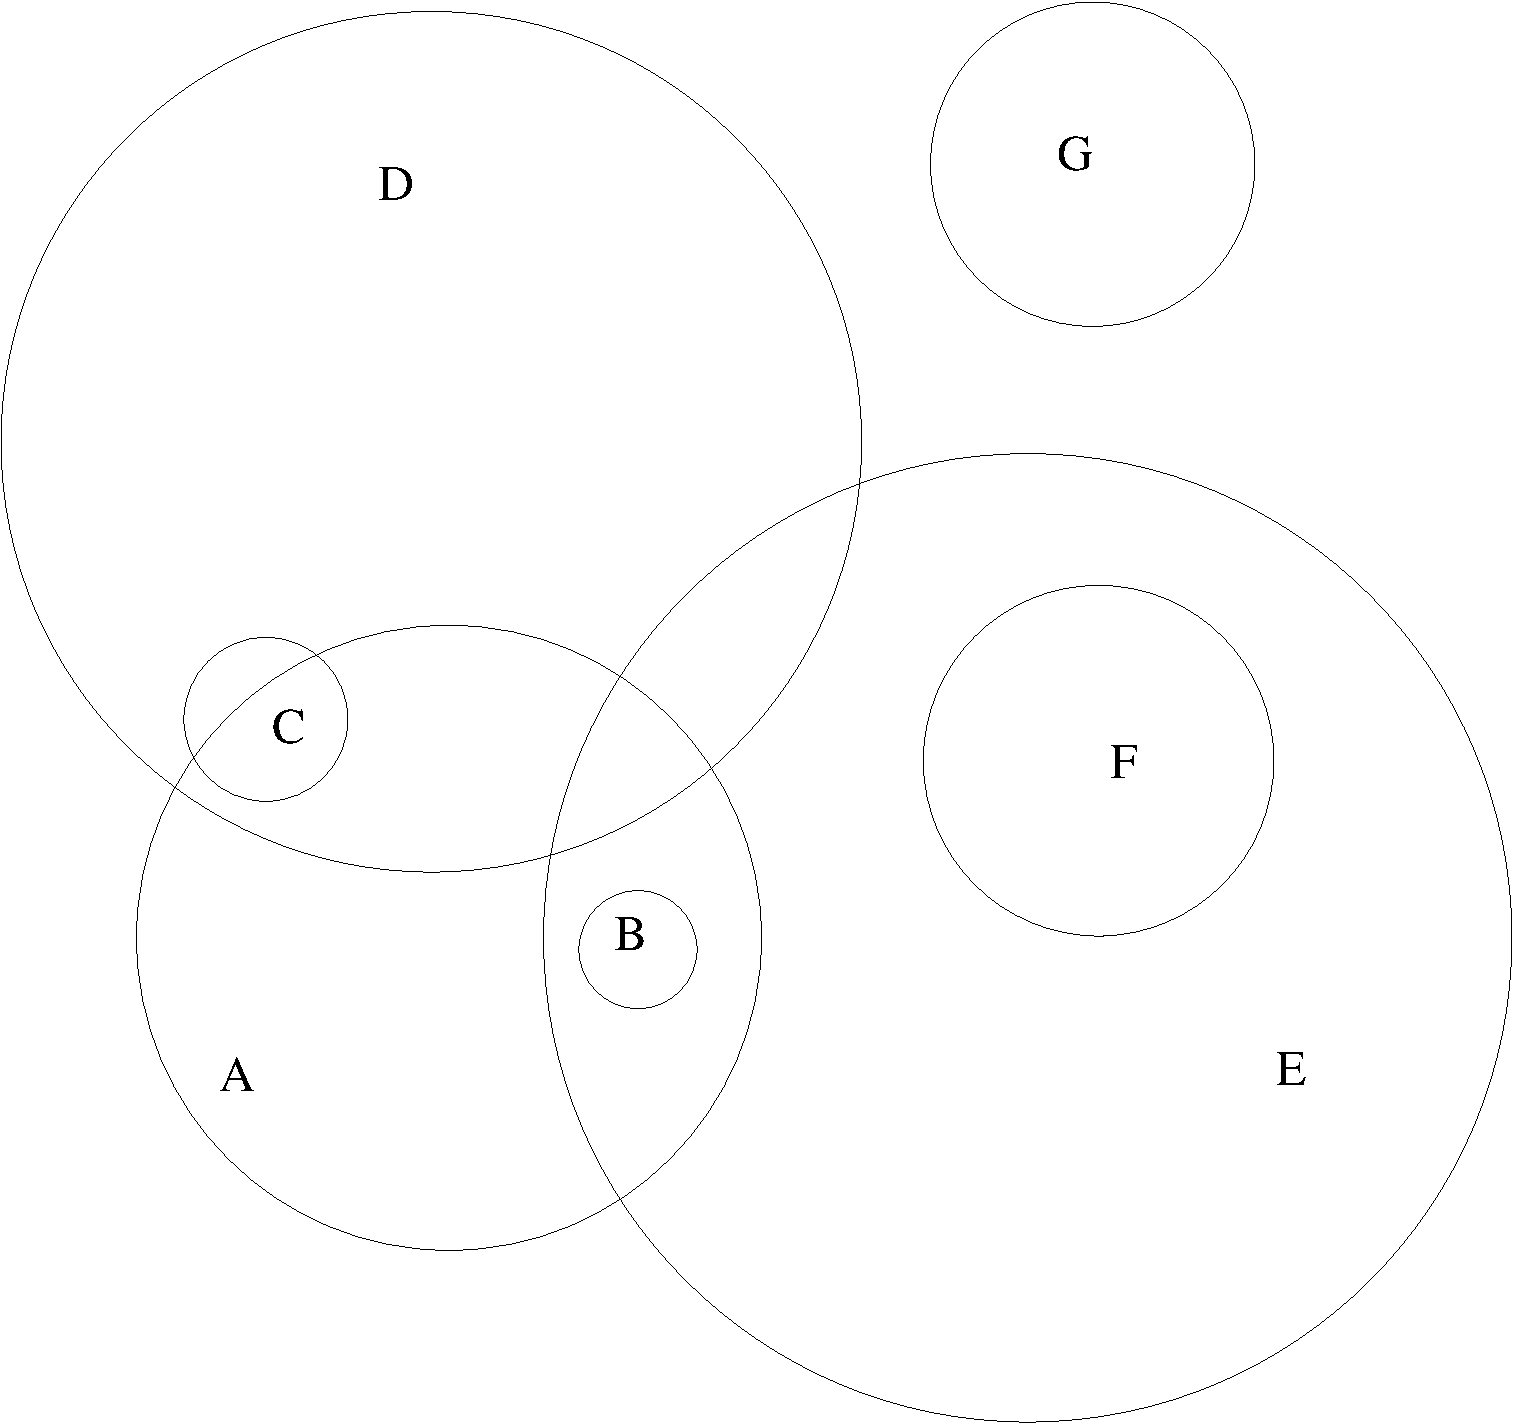
\includegraphics[width=0.65\linewidth,keepaspectratio=]{figures/vennproblemsheet.pdf}
\end{center}

Betrachten Sie das obenstehende Venn-Diagramm, und bestimmen Sie jeweils den Wahrheitswert der folgenden Aussagen:\\
\parbox{0.5\textwidth}{
\begin{enumerate}
\item $A\subseteq B$
\item $B\subset A$
\item $B\cap C=\emptyset$
\item $B\subseteq E$
\item $B\subset(A\cap E)$
\item $C\subseteq(A\cap D)$
\item $C\subseteq(A\cup D)$
\item $F\subset(E\backslash D)$
\end{enumerate}}\parbox{0.5\textwidth}{
\begin{enumerate}\setcounter{enumi}{8}
\item $C\subseteq(D\backslash A)$
\item $C\cap(D\backslash A)=\emptyset$
\item $F\subset(E\cup G)$
\item $C\subset(D\backslash E)$
\item $(C\cap A)\subset D$
\item $G\cup F=\emptyset$
\item $F\backslash E=\emptyset$
\item $(B\cap C)\subseteq (D\cap G)$
\end{enumerate}}



\question{{\it Mengentheoretische Gesetze}}

Beweisen Sie folgende Mengentheoretische Gesetze jeweils mit Hilfe des Extensionalitätsprinzips sowie der aussagenlogischen Gesetze aus Aufgabe 1:
\begin{enumerate}
\item $(A\cap(B\cap C))=((A\cap B)\cap C)$
\item $(A\cup(B\cup C))=((A\cup B)\cup C)$
\item $(A\cap(B\cup C))=((A\cap B)\cup(A\cap C))$
\item $(A\cup(B\cap C))=((A\cup B)\cap(A\cup C))$
\end{enumerate}



\question{{\it Zum Nachdenken und Diskutieren}}

\begin{enumerate}
\item Machen Sie sich den Unterschied zwischen dem umgangssprachlichen Gebrauch von ``wenn \ldots dann \ldots'' und der Bedeutung des aussagenlogischen $p\Rightarrow q$ an Beispielen wie ``Wenn Du Deine Suppe aufißt, bekommst Du Dessert.'' klar.
\item Erklären Sie ihrem Banknachbarn Ihre Einsichten.
\item Wiederholen Sie die beiden vorangehenden Schritte für umgangssprachlichen ``oder'' und aussagenlogisches $\vee$. Welche Unklarheit in der Bedeutung hat das umgangssprachliche ``oder''?
\end{enumerate}

\question{{\it Teilbarkeit und Division mit Rest}}

Bestimmen Sie jeweils, ob eine der beiden angegebenen natürlichen Zahlen die andere teilt. Falls nicht, geben Sie jeweils den Rest bei Division der größeren durch die kleinere Zahl an.\\
\parbox{0.5\textwidth}{\begin{enumerate}
\item $5$, $15$    %5 teilt 15
\item $50$, $67$   %67 = 1*50 + 17, Rest 17
\item $3$, $102$   %3 teilt 102
\item $129$, $129$   %129 teilt sich selbst
\end{enumerate}}\parbox{0.5\textwidth}{\begin{enumerate}\setcounter{enumi}{4}
\item $25$, $505$  %505 = 20*25 + 5, Rest 5
\item $1024$, $9$  %1024 = 113*9 + 7, Rest 7
\item $10023$, $3$ %3 teilt 10023
\item $978654321081$, $8$ %8 teilt 1000, also Rest 1
\end{enumerate}}



\question{{\it Primzahlen und Faktorisierung}}

Bestimmen Sie für die folgenden Zahlen jeweils, ob es sich um Primzahlen handelt. Falls nicht, geben Sie jeweils die Faktorisierung in Primzahlen an.\\
\parbox{0.5\textwidth}{\begin{enumerate}
\item $3$    %prim
\item $1$    %nicht prim, 1
\item $1024$ %nicht prim, 2^10
\item $243$  %nicht prim, 3^5
\end{enumerate}}\parbox{0.5\textwidth}{\begin{enumerate}\setcounter{enumi}{4}
\item $3600$ %nicht prim, 2^4 3^2 5^2
\item $3060$ %nicht prim, 2^2 3^2 5 17
\item $137$  %prim
\item $237$  %nicht prim, 3 79
\end{enumerate}}


\pagebreak


\question{{\it Kürzen von Brüchen}}

Kürzen Sie folgende Brüche jeweils soweit wie möglich ($a$, $b$, $c$ seien jeweils beliebige, paarweise teilerfremde, natürliche Zahlen ungleich Null):\\
\parbox{0.5\textwidth}{\begin{enumerate}
\item $\frac{15}{25}$
\item $\frac{720a^2}{12ab}$
\item $\frac{48(a^2-b^2)}{6a+6b}$
\item $\frac{ab+ac}{(a+b)^2-b^2}$
\end{enumerate}}\parbox{0.5\textwidth}{\begin{enumerate}\setcounter{enumi}{4}
\item $\frac{(a-b)^3+(b^3-a^3)}{36a}$
\item $\frac{a^{32}-1024}{a^{16}-32}$
\item $\frac{a^2+1024}{a+1024}$
\item $\frac{2310(a^4-b^2)}{4641(a^2+b)}$
\end{enumerate}}


\question{{\it Rechnen mit rationalen Zahlen}}

Formen Sie die folgenden Ausdrücke jeweils so um, dass nur ein soweit wie möglich gekürzter Bruch übrigbleibt:\\
\parbox{0.5\textwidth}{\begin{enumerate}
\item $\frac{7}{3}+\frac{15}{24}$
\item $3\cdot\frac{2}{9}-\frac{21+7}{4^2}$
\item $\frac{4}{7}\cdot\frac{49}{12}$
\item $\left(2+\frac{1}{137}\right)^3$
\end{enumerate}}\parbox{0.5\textwidth}{\begin{enumerate}\setcounter{enumi}{4}
\item $\frac{49}{3}-\frac{150-3}{21}$
\item $\frac{100}{13}\cdot\frac{196}{10}$
\item $\frac{1+2+3}{2^{10}}\cdot\frac{8^2}{3!}$
\item $\frac{9}{11}/\frac{121}{27}$
\end{enumerate}}



\question{{\it Rationale und Irrationale Zahlen}}

Entscheiden Sie jeweils, ob die folgenden Zahlen rational oder irrational sind, und beweisen Sie gegebenenfalls die Irrationalität:\\
\parbox{0.5\textwidth}{\begin{enumerate}
\item $\frac{5}{2}$ %rational
\item $\sqrt{37}$   %irrational, Beweis wie sqrt(2), da 37 prim
\item $\sqrt{36}$   %=6, rational
\end{enumerate}}\parbox{0.5\textwidth}{\begin{enumerate}\setcounter{enumi}{3}
\item $\frac{1}{\sqrt{2}}$ %irrational, da sonst rational*irrational=1 sein muesste, im Widerspruch zur Koerpereigenschaft von \Qset
\item $\frac{1+\sqrt{5}}{2}$ %irrational, da rational+irrational irrational sein muss (sonst Widerspruch zur Koerpereigenschaft von \Qset)
\item $\frac{(1+\sqrt{5})^2+(1-\sqrt{5})^2}{(1+\sqrt{5})^2-2(1+\sqrt{5})}$ %=12/4=3, rational
\end{enumerate}}



\question{{\it Potenzen und Logarithmen}}

Vereinfachen Sie folgende Ausdrücke jeweils unter Verwendung der Potenz- und
Logarithmengesetze soweit, dass höchstens noch eine Potenz oder ein Logarithmus im Ergebnis auftritt ($a,b,c>0$, $n,m\in\Nset$):\\
\parbox{0.5\textwidth}{\begin{enumerate}
\item $\log_a b + \log_a c -\log_b b^c$
\item $\log_b a \cdot \log_a b$
\item $\log_2 1024 - \log_5 125$
\item $2^{\log_3 9}$
\end{enumerate}}\parbox{0.5\textwidth}{\begin{enumerate}\setcounter{enumi}{4}
\item $a^n b^n c^{-n}$
\item $(a^n z^{-n})^{1/(n+1)}$
\item $a^m a^n$
\item $(a+b)^m c^m$
\end{enumerate}}


\pagebreak


\question{{\it Wissenschaftliche Notation}}

Schreiben Sie folgende Zahlen jeweils in wissenschaftlicher Notation bzw. als Dezimalbruch:\\
\parbox{0.5\textwidth}{\begin{enumerate}
\item $0,003$
\item $1024$
\item $1\,000\,000\,000$
\item $0,00000000723455$
\end{enumerate}}\parbox{0.5\textwidth}{\begin{enumerate}\setcounter{enumi}{4}
\item $1,2\times 10^{-5}$
\item $9,931\times 10^9$
\item $7,04\times 10^{-1}$
\item $1,01\times 10^{3}$
\end{enumerate}}



\question{{\it Komplexe Zahlen}}

Bestimmen Sie für folgende komplexe Zahlen $z$ jeweils Re~$z$, Im~$z$, $|z|$, $\arg(z)$ und $z^*$ ($a$ und $b$ seien jeweils beliebige reelle Zahlen):\\
\parbox{0.5\textwidth}{\begin{enumerate}
\item $z=a+bi$
\item $z=4-4i$
\item $z=13a$
\item $z=(a^6+5)i$
\end{enumerate}}\parbox{0.5\textwidth}{\begin{enumerate}\setcounter{enumi}{4}
\item $z=\sqrt{3}-3i$
\item $z=\sqrt{2}\rme^{\frac{\pi}{4}i}$
\item $z=\rme^{\frac{\pi}{6}i}$
\item $z=17\rme^{3\pi i}$
\end{enumerate}}



\question{{\it Rechnen mit komplexen Zahlen}}

Formen Sie die folgenden Ausdrücke jeweils in die Form $a+bi$ mit $a,b\in\Rset$ um:\\
\parbox{0.4\textwidth}{\begin{enumerate}
\item $(3+5i)-(4-2i)$
\item $\frac{1-2i}{3}+\frac{3+5i}{2}$
\item $(1+2i)^{-1}$
\item $(1+i)(1-i)$
\item $(12+3\sqrt{2}i)\left(\frac{1}{3}-\sqrt{2}i\right)$
\item $\rme^{\frac{\pi}{2}i}-5\left(2+\rme^{\pi i}\right)$
\item $\frac{1+i}{1-i}$
\end{enumerate}}\parbox{0.6\textwidth}{\begin{enumerate}\setcounter{enumi}{7}
\item $\frac{5}{3+4i}$
\item $(1+i)\rme^{\frac{3\pi}{4}i}$
\item $\left(\frac{(1+i)^4}{2-2i}\right)^2$
\item $\left(\rme^{\frac{\pi}{4}i}-1\right)\left(\rme^{\frac{\pi}{4}i}+\frac{1}{2}+\frac{\sqrt{3}}{2}i\right)\left(\rme^{\frac{\pi}{4}i}-\rme^{\frac{2\pi i}{3}}\right)$
\item $\rme^{\frac{\pi i}{8}}+\rme^{\frac{19\pi i}{24}}+\rme^{-\frac{13\pi i}{24}}$
\end{enumerate}}



\question{{\it Trigonometrische Identitäten}}

Leiten Sie die folgenden trigonometrischen Identitäten jeweils mit Hilfe der Euler-Formel $\rme^{i\alpha}=\cos\alpha+i\sin\alpha$ her:\\
\parbox{0.5\textwidth}{\begin{enumerate}
\item $\sin(2\alpha)=2\cos\alpha\sin\alpha$
\item $\cos(3\alpha)=\cos^3\alpha-3\cos\alpha\sin^2\alpha$
\item $\sin(\alpha+\beta)=\sin\alpha\cos\beta+\sin\beta\cos\alpha$
\end{enumerate}}\parbox{0.5\textwidth}{\begin{enumerate}\setcounter{enumi}{3}
\item $\cos(\alpha-\beta)=\cos\alpha\cos\beta+\sin\alpha\sin\beta$
\item $\sin^2(\alpha)=\frac{1}{2}-\frac{1}{2}\cos(2\alpha)$
\item $\sin(\alpha+\beta)\sin(\alpha-\beta)=\sin^2\alpha-\sin^2\beta$
\end{enumerate}}



\pagebreak



\question{{\it Beweis mittels vollständiger Induktion}}

Beweisen Sie folgenden Aussagen jeweils mittels vollständiger Induktion:\\
\parbox{0.5\textwidth}{\begin{enumerate}
\item $\forall n\in\Nset~n^2=\sum\limits_{k=0}^{n-1} (2k+1)$
\item $\forall n\in\Nset~ 2^n-1=\sum\limits_{k=0}^{n-1} 2^k$
\item $\forall n\in\Nset~\sum\limits_{k=0}^{n-1} 3^k = \frac{3^n-1}{2}$ 
\end{enumerate}}\parbox{0.5\textwidth}{\begin{enumerate}\setcounter{enumi}{3}
\item $\forall n\in\Nset~\sum\limits_{k=0}^n k=\frac{n(n+1)}{2}$ 
\item $\forall n\in\Nset~\sum\limits_{k=0}^{n-1} (2k+1)^2=\frac{n(2n-1)(2n+1)}{3}$
\item $\forall n\in\Nset~\forall x\in[0;\infty)~(1+x)^n\ge 1+nx$
\end{enumerate}}


\question{{\it Polynomdivision}}

Führen Sie für die folgenden Paare von Polynomen jeweils die Polynomdivision durch.
\begin{enumerate}
\item $(x^3-x^2-5x-3)$, $(3-x)$
\item $(x^4+3x^3+4x^2+3x+1)$, $(x^2+x+1)$
\item $(6 x^4-12 x^3+37 x^2-48 x+45)$, $(2 x^2-4 x+4)$
\item $(x^5+4 x^4-9 x^3-40 x^2-4 x+48)$, $(x^2+4x+4)$
\item $(x^5+4 x^4-9 x^3-40 x^2-4 x+48)$, $(x^3-13 x+12)$
\item $(2 x^8+4 x^7+3 x^6-5 x^5-16 x^4-13 x^3+4 x^2-4 x+18)$, $(x^3+x-4)$
\item $(x^8-4 x^7+14 x^6-4 x^5+13 x^4+x^2-3)$, $(x^5-4 x^4+13 x^3)$
\item $(x^{10}-1)$, $(1 - x + x^2 - x^3 + x^4)$
\end{enumerate}



\question{{\it Faktorisierung von Polynomen}}

Bestimmen Sie für die folgenden Polynome jeweils alle reellen Nullstellen und überprüfen Sie, ob das Polynom über $\Rset$ in Linearfaktoren zerfällt. Falls nicht, geben Sie die verbleibenden quadratischen Faktoren an und bestimmen Sie die zugehörigen komplexen Nullstellen.\\
\parbox{0.5\textwidth}{\begin{enumerate}
\item $x^2-2x+1$
\item $x^2+2x+1$ 
\item $x^2+4$
\item $x^3+9x$
\end{enumerate}}\parbox{0.5\textwidth}{\begin{enumerate}\setcounter{enumi}{4}
\item $x^3-13 x+12$
\item $x^3-5 x^2+7 x-3$
\item $6 x^4-12 x^3+36 x^2-48 x+48$ 
\item $x^8 - 2 x^4 + 1$
\end{enumerate}}

\pagebreak




\end{questions}

\end{document}
